\documentclass[usenames,dvipsnames]{beamer}

\usetheme[
	progressbar=frametitle,
	titleformat section=smallcaps,
	subsectionpage=progressbar
]{metropolis}

\input{version}

% cSpell:disable

% CLI arguments

\ifdefined\generatenotes%
	\newcommand{\notesOption}{show notes on second screen}%
\else
	\newcommand{\notesOption}{hide notes}%
\fi

% packages

\usepackage{pgfpages}
\usepackage{booktabs}
\usepackage{bm}
\usepackage{mathtools}
\usepackage{listings}
\usepackage{fancybox}
\usepackage{bm}
\usepackage{multicol}
\usepackage{xpatch}
\usepackage{hyperref}
\usepackage{hyperxmp}
\usepackage{multirow}
\usepackage{xparse}
\usepackage{caption}

\usepackage[
	backend=biber,
	style=alphabetic,
	sorting=ynt
]{biblatex}

\usepackage[printwatermark]{xwatermark}
\usepackage{ifthen}

% settings

\graphicspath{{./graphics/}}

\setbeameroption{\notesOption}

\makeatletter
\let\@@magyar@captionfix\relax % chktex 21
\makeatother

\logo{
	\includegraphics[
		width=1cm,
		keepaspectratio
	]{logo.eps}\hspace{\dimexpr\paperwidth-36pt}\vspace{-30pt}
}

\addbibresource{bibfile.bib}

\makeatletter
	\def\beamer@framenotesbegin{% at beginning of slide
		\usebeamercolor[fg]{normal text} 
			\gdef\beamer@noteitems{}%
			\gdef\beamer@notes{}% 
	}
\makeatother

\hypersetup{
	colorlinks=true,
	linkcolor=magenta,
	urlcolor=cyan,
	citecolor=blue,
	pdfpagemode=FullScreen,
	pdfdisplaydoctitle=true,
	pdfmenubar=false,
	pdfpagelayout=SinglePage
}

\captionsetup[figure]{labelformat=empty}

\definecolor{CardinalRed}{RGB}{172,29,55} 
\definecolor{Tangerine}{RGB}{247,148,30} 

\setbeamercolor{alerted text}{fg=CardinalRed}
\setbeamercolor{example text}{fg=Tangerine}
{
	\usebeamercolor[fg]{alerted text}
	\usebeamercolor[fg]{example text}
}

% definitions

\newcommand{\BigO}[1]{\mathcal{O}\left(#1\right)}
\newcommand{\BigOmega}[1]{\Omega\left(#1\right)}

\DeclarePairedDelimiter\ceil{\lceil}{\rceil}
\DeclarePairedDelimiter\floor{\lfloor}{\rfloor}

\newsavebox{\mybox}
\newsavebox{\tablebox}

\xpatchbibmacro{name:andothers}{%
	\bibstring{andothers}%
}{%
	\bibstring[\emph]{andothers}%
}{}{}

\newsavebox\watermark%
\savebox\watermark{\tikz[color=gray,opacity=0.02]\node{\wm};}
\newwatermark*[
	allpages,
	angle=0,
	scale=3,
	xpos=0,
	ypos=-25
]{\usebox\watermark}

\makeatletter
	\newcommand{\manuallabel}[2]{\def\@currentlabel{#2}\label{#1}} % chktex 21
\makeatother

\newenvironment<>{fixblock}[1]{%
	\begin{block}{#1}
		\vspace{0pt}
		#2
}{
	\end{block}
}


\title{Dissertation Defense}

\subtitle{
	Secure and Efficient Query Processing in Outsourced Databases \\
	{\small Range Queries~\cite{ore-benchmark-17, epsolute}, Point Queries~\cite{epsolute}, \knn{} Queries}
}

\date{Built from \href{https://git.dbogatov.org/bu/defense/presentation/commit/\version}{\emph{\version}} on \today}

\author{Dmytro Bogatov \\ \email{dmytro@bu.edu}}

\institute{Boston University \\ Graduate School of Arts and Sciences \\ Department of Computer Science}

\def\wm{
\includegraphics[keepaspectratio, width=0.1\textwidth]{coat-of-arms-1}}


\begin{document}

	\nobibliography*

	\maketitle

	\setbeamercovered{transparent}

	\section{Introduction and Background}

	\begin{frame}{Motivation and overview}

		\begin{itemize}
			\item<1-> With vast amounts of data, organizations choose to use cloud
			\item<1-> \alert{Challenge:} solutions must be both \textbf{secure} and \textbf{efficient}
			\item<2-> Query types: \texttt{SELECT * FROM t1 }
				\begin{itemize}
					\item<1,2,6-> Point queries: \texttt{WHERE zip = '02215'}
					\item<1,3,6-> Range queries: \texttt{WHERE age BETWEEN 18 AND 65}
					\item<1,4,6-> \knn{} queries: \texttt{ORDER BY location <-> '(29.9691,-95.6972)' LIMIT 5} % chktex 36
					\item<1,5,6-> \texttt{JOIN} / \texttt{GROUP BY} queries: \texttt{INNER JOIN t2 ON (t1.k = t2.k) GROUP BY zip}
				\end{itemize}
			\item<6-> Security models for an outsourced database system
				\begin{itemize}
					\item<1-5,6> \textbf{Snapshot} adversary: steal the hard drive and RAM snapshot % chktex 8
					\item<1-5,7> \textbf{Persistent} adversary: continuously monitor the entire server % chktex 8
				\end{itemize}
		\end{itemize}

	\end{frame}

	\begin{frame}{My work}

		\begin{block}{Proposed thesis structure}

			\vspace*{-1ex}

			\begin{itemize}[label={}]
				\setlength\itemsep{-0ex}

				\item<1> \bibentry{ore-benchmark-17}

					\begin{itemize}[label={}]
						\item \small Model: \alert{snapshot}, query type: \alert{range} \normalsize
					\end{itemize}

				\item<2> \bibentry{epsolute}

					\begin{itemize}[label={}]
						\item \small Model: \alert{persistent}, query type: \alert{point} and \alert{range} \normalsize
					\end{itemize}

			\end{itemize}

			\begin{columns}[T,onlytextwidth]
				\column{0.44\textwidth}

					\vspace*{-0.5ex}

					\begin{itemize}[label={}]
						\item<3> In-progress: Private \knn{} queries

						\begin{itemize}[label={}]
							\item \small Model: \alert{snapshot}, query type: \alert{\knn{}} \normalsize
						\end{itemize}

						\item<4> In-progress: Oblivious \texttt{JOIN} queries

						\begin{itemize}[label={}]
							\item \small Model: \alert{persistent}, query type: \alert{\texttt{JOIN}} \normalsize
						\end{itemize}

					\end{itemize}

				\column{0.56\textwidth}

					\visible<5->{
						\bibentry{bogatov-idemix-2020}
					}

			\end{columns}

		\end{block}

	\end{frame}

	\section{A comparative evaluation of order-revealing encryption schemes and secure range-query protocols~\cite{ore-benchmark-17}}

	\begin{frame}{Survey of OPE/ORE schemes~\cite{ore-benchmark-17}}

		\begin{columns}[T,onlytextwidth]
			\column{0.5\textwidth}

				\begin{block}{The problem}

					\begin{itemize}
						\item Model: \alert{snapshot}, query type: \alert{range}
						\item Performance / security tradeoff
						\item Heterogeneous security definitions and leakage profiles
						\item \textbf{Performance of the schemes not well-understood}
						\begin{itemize}
							\item Some were not even implemented
							\item Prototype implementation at best
							\item Not benchmarked against one another
							\item Use different primitive implementations
						\end{itemize}
					\end{itemize}

				\end{block}

			\column{0.5\textwidth}

				\onslide<2->{
					\begin{block}{Our solution}

						\begin{itemize}
							\item Analyzed security and leakages of the constructions under a common framework
							\item Analyzed theoretically performance of the constructions
							\item \textbf{Implemented and run experiments}
							\begin{itemize}
								\item Implemented 5 OPE / ORE schemes and 5 range query protocols
								\item Used same language, framework and primitive implementations
								\item Benchmarked primitives execution times
								\item Counted primitives and I/O usage
							\end{itemize}
						\end{itemize}

					\end{block}
				}

		\end{columns}

	\end{frame}

	\begin{frame}{OPE / ORE schemes}

		\begin{adjustbox}{width=\linewidth}
			\begin{tabular}{ l c c c c c }

				\toprule

				\multirow{2}{*}{Scheme}						& \multicolumn{2}{c}{\onslide<2->{Primitive usage}}																						& \onslide<2->{Ciphertext size,}																& \onslide<2->{Leakage}																\onslide<2->{\\ \cline{2-3}}
				\rule{0pt}{10pt}							& \onslide<2->{Encryption}													& \onslide<2->{Comparison}									& \onslide<2->{or state size}																	& \onslide<2->{(In addition to inherent total order)}								\\

				\toprule

				BCLO~\cite{crypt-db-ope}					& \onslide<3->{$\bm{n}$ \textbf{HG}}										& \onslide<3->{none}										& \onslide<3->{$2n$}																			& \onslide<3->{\textbf{$\approx$ Top half of the bits}}								\\

				\midrule

				CLWW~\cite{practical-ore}					& \onslide<3->{$n$ PRF} 													& \onslide<3->{none}										& \onslide<3->{$2n$}																			& \onslide<3->{\textbf{Most-significant differing bit}}								\\

				\midrule

				\multirow{3}{*}{Lewi-Wu~\cite{lewi-ore}}	& \onslide<3->{\boldmath{} $\nicefrac{2n}{d}$ \unboldmath{} \textbf{PRP}}	& \onslide<3->{\multirow{3}{*}{$\frac{n}{2d}$ Hash}}		& \onslide<3->{\multirow{3}{*}{$\frac{n}{d} \left(\lambda + n + 2^{d + 1} \right) + \lambda$}}	& \onslide<3->{\multirow{3}{*}{Most-significant differing block}}					\\
															& \onslide<3->{$2 \frac{n}{d} \left( 2^d + 1 \right)$ PRF}					&															&																								&																					\\
															& \onslide<3->{$\frac{n}{d} 2^d$ Hash}										&															&																								&																					\\

				\midrule

				\multirow{3}{*}{CLOZ~\cite{adam-ore-v2}}	& \onslide<3->{$n$ PRF}														& \onslide<3->{\multirow{3}{*}{$\bm{n^2}$ \textbf{PPH}}}	& \onslide<3->{\multirow{3}{*}{$n \cdot h$}}													& \onslide<3->{\multirow{3}{*}{Equality pattern of most-significant differing bit}}	\\
															& \onslide<3->{$n$ PPH}														&															&																								&																					\\
															& \onslide<3->{1 PRP}														&															&																								&																					\\

				\midrule

				FH-OPE~\cite{fh-ope}						& \onslide<3->{1 Traversal}													& \onslide<3->{3 Traversals}								& \onslide<3->{$\bm{3 \cdot n \cdot N}$}														& \onslide<3->{Insertion order}														\\

				\bottomrule

			\end{tabular}
		\end{adjustbox}

	\end{frame}

	\begin{frame}{Range query protocols}

		\begin{adjustbox}{width=\linewidth}
			\begin{tabular}{ l c c c c c c }

				\toprule

				\multirow{2}{*}{Protocol}						& \multicolumn{2}{c}{\onslide<2->{{\IO} requests}}																																& \multirow{2}{*}{\onslide<2->{Leakage}}	& \multicolumn{2}{c}{\onslide<2->{Communication (result excluded)}}																&	\onslide<2->{\\ \cline{2-3} \cline{5-6}}
				\rule{0pt}{10pt}								& \onslide<2->{Construction}									& \onslide<2->{Query}																							&											& \onslide<2->{Construction}									& \onslide<2->{Query} 											&	\\

				\toprule

				{\BPlus} tree with ORE							& \onslide<3->{$\log_B \frac{N}{B}$}							& \onslide<3->{$\log_B \frac{N}{B} + \frac{r}{B}$}																& \onslide<3->{\textbf{Same as ORE}}		& \onslide<3->{$1$}												& \onslide<3->{$1$}												&	\\
				\midrule

				Kerschbaum~\cite{florian-protocol}				& \onslide<3->{$\bm{\frac{N}{B}}$}								& \onslide<3->{$\log_2 \frac{N}{B} + \frac{r}{B}$}																& \onslide<3->{\textbf{Total order}}		& \onslide<3->{$\log_2 N$}										& \onslide<3->{$\log_2 N$}										&	\\

				\midrule

				POPE~\cite{pope} warm							& \multirow{2}{*}{\onslide<3->{$1$}}							& \onslide<3->{$\log_L \frac{N}{B} + \frac{r}{B}$}																& \onslide<3->{\textbf{Partial order}}		& \multirow{2}{*}{\onslide<3->{$1$}}							& \onslide<3->{$\log_L N$}										&	\\

				POPE~\cite{pope} cold							& 																& \onslide<3->{$\bm{{\nicefrac{N}{B}}}$}																		& \onslide<3->{Fully hiding}				& 																& \onslide<3->{$\bm{N}$}										&	\\

				\midrule

				Logarithmic-BRC~\cite{practical-range-search}	& \onslide<3->{\textbf{---}}									& \onslide<3->{$\bm{r}$}																						& \onslide<3->{Same as SSE}					& \onslide<3->{\textbf{---}}									& \onslide<3->{$\log_2 N$}										&	\\

				\midrule

				\multirow{2}{*}{ORAM}							& \multirow{2}{*}{\onslide<3->{$\bm{{ \log^2 \frac{N}{B} }}$}}	& \multirow{2}{*}{\onslide<3->{$\bm{{ \log_2 \frac{N}{B} \left( \log_B \frac{N}{B} + \frac{r}{B} \right) }}$}}	& \onslide<3->{Fully hiding}				& \multirow{2}{*}{\onslide<3->{$\bm{{ \log^2 \frac{N}{B} }}$}}	& \multirow{2}{*}{\onslide<3->{$\bm{{ \log^2 \frac{N}{B} }}$}}	&	\\
																&																&																												& \onslide<3->{(access pattern)}			&																&																&	\\

				\bottomrule

			\end{tabular}
		\end{adjustbox}

	\end{frame}

	\begin{frame}{One of the experimental results}

		\begin{figure}[h]
			\centering
			\includegraphics[width=0.6\textwidth]{protocol-charts-qios}
			\caption{Query stage number of I/O requests}
		\end{figure}

	\end{frame}

	\section{\epsolute{}: Efficiently Querying Databases While Providing Differential Privacy~\cite{epsolute}}

	\begin{frame}[label={frame:epsolute-motivation}]

		\frametitle{Motivation}

		\begin{block}{The problem}

			\begin{itemize}
				\item<1-> Previous solutions work in the snapshot model (adversary steals the hard drive)
				\item<1->
					What about \textbf{persistent} adversary (malicious script with \texttt{root} permissions)? \\
					\begin{small}
						Model: \alert{persistent}, query type: \alert{point} and \alert{range}
					\end{small}
				\item<1-> Need to protect \alert{access pattern} and \alert{communication volume}
				\item<2->
					Using ORAM to hide the access pattern \\
					\begin{small}
						Expensive, each request costs $\bigO{\log n}$ \hyperlink{frame:appendix:oram}{\beamerskipbutton{ORAM definition}}
					\end{small}
				\item<3->
					Adding fake records (noise) to the answer to hide the result size \\
					\begin{small}
						How much noise to add to have a guarantee and the least overhead? \\
						Adding a constant or a uniformly sampled noise is not an option \\
						Differential Privacy!
					\end{small}
			\end{itemize}

		\end{block}

	\end{frame}

	\begin{frame}{Differential Privacy, LPA and Sanitization}

		\begin{definition}[\alert{Differential Privacy}, adapted from~\cite{our-data-ourselves, differential-privacy-original}]
			\justify%

			A randomized algorithm \algo{A} is $(\epsilon, \delta)$-differentially private if for all $\database_1 \sim \database_2 \in \searchKeyDomain^\dataSize$, and for all subsets $\mathcal{O}$ of the output space of \algo{A},
			\[
				\probability{ \algo{A}{ \database_1 } \in \mathcal{O} } \leq \exp(\epsilon) \cdot \probability{ \algo{A}{ \database_2 } \in \mathcal{O} } + \delta \; .
			\]
		\end{definition}

		\pause%

		\begin{columns}[T,onlytextwidth]
			\column{0.6\textwidth}

				\begin{block}{How to make sense of it?}
					\begin{itemize}
						\item<2->
							Differential Privacy is a property of an algorithm \\
							\begin{small}
								What about $\epsilon$ and $\delta$?
							\end{small}
						\item<3->
							How to construct such an algorithm? \\
							\begin{small}
								Laplace Perturbation Method!
							\end{small}
						\item<4->
							What if negative value is sampled? \\
							\begin{small}
								Cannot truncate one side, must shift entire distribution
							\end{small}
					\end{itemize}
				\end{block}

			\column{0.4\textwidth}

				\centering
				\includegraphics<5->[width=1.0\linewidth]{sanitizer}

		\end{columns}

	\end{frame}

	\begin{frame}{Differentially Private Outsourced Database System}

		\begin{definition}[\alert{Computationally Differentially Private Outsourced Database System (CDP-ODB)}]
			\justify%

			We say that an outsourced database system \protocol{} is $(\epsilon, \delta)$-computationally differentially private (a.k.a.~CDP-ODB) if for every polynomial time distinguishing adversary \adversary{}, for every neighboring databases $\database \sim \database^\prime$, and for every query sequence $\fromNtoM{\query}{1}{m} \in \querySet^m$ where $m = \mathsf{poly}(\lambda)$,

			\begin{multline*}
				\probability{\adversary \left( 1^\lambda, \view{\protocol, \server}{\database, \fromNtoM{\query}{1}{m}} \right) = 1 } \leq \\
				\exp{\epsilon} \cdot \probability{\adversary \left( 1^\lambda, \view{\protocol ,\server}{\database^\prime, \fromNtoM{\query}{1}{m}} \right) = 1} + \delta + \negl \; ,
			\end{multline*}
			the probability is over the randomness of the distinguishing adversary \adversary{} and the protocol \protocol{}.
		\end{definition}

		\pause%

		Note:
		\begin{itemize}
			\item Entire view of the adversary is DP-protected
			\item Implies protection against \textbf{communication volume} and \textbf{access pattern} leakages
			\item Query sequence $\fromNtoM{\query}{1}{m} \in \querySet^m$ is fixed (more on that next)
			\item $\negl$ needed for the computational (as opposed to information-theoretical) DP definition
		\end{itemize}

	\end{frame}

	\begin{frame}{On impossibility of adaptive queries}

		\begin{block}{Why is the query sequence $\fromNtoM{\query}{1}{m} \in \querySet^m$ fixed?}
			\justify%

			\begin{itemize}
				\item<1-> Suppose neighboring medical databases differ in one record with a rare diagnosis ``Alzheimer's disease''
				\item<2-> A medical professional, who is \textbf{a user, not an adversary} queries the database
					\begin{itemize}
						\item
							for that diagnosis first \\
							\texttt{SELECT name FROM patients WHERE condition = 'ALZ'} % chktex 32

						\item
							if there is a record, she queries the senior patients next \\
							\texttt{SELECT name FROM patients WHERE age >= 65}

						\item
							otherwise she queries the general population, resulting in many more records \\
							\texttt{SELECT name FROM patients}
					\end{itemize}
				\item<3-> \alert{Adversary can know the answer to the first query by observing result size of the second}
				\item<3-> Efficient system cannot return nearly the same number of records in both cases, thus, the adversary can distinguish
			\end{itemize}

		\end{block}

	\end{frame}

	\begin{frame}{Single-Threaded \epsolute{}}

		\begin{block}{Single-Threaded \epsolute{} protocol}

			\vspace*{2ex}
			\centering
			\includegraphics[width=\textwidth]{dp-oram}

		\end{block}

	\end{frame}

	\begin{frame}{Parallel \epsolute{}}

		\onslide<1->{
			\begin{itemize}
				\item
					Single-threaded version is prohibitively slow, must parallelize \\
					\begin{small}
						Assume single-threaded solution generates $r = \num{1500}$ real and $f = \num{500}$ noisy records
					\end{small}

				\item Split \user{} and \server{} state into \oramsNumber{} ORAMs, run as separate machines (assume $\oramsNumber = 4$)
				\item Partition records randomly (by ID) into \oramsNumber{} partitions, generate \oramsNumber{} inverted indexes
				\item What to do about \serverDS{}?
			\end{itemize}
		}

		\begin{columns}[T]
			\begin{column}{0.5\textwidth}

				\onslide<2->{
					\begin{block}{No-$\gamma$ method: \serverDS{} per ORAM}

						\begin{itemize}[leftmargin=*]
							\item Composition of disjoint datasets: take max $\epsilon$
							\item Each ORAM incurs noise comparable to $f$
							\item Win by splitting ORAM work $r$ into \oramsNumber{} partitions and lose by multiplying noise $f$ times \oramsNumber{}
							\item That is, each ORAM is processing $\frac{r}{\oramsNumber} + f = \num{875}$ records in parallel
						\end{itemize}

					\end{block}
				}

			\end{column}

			\begin{column}{0.5\textwidth}

				\onslide<3->{
					\begin{block}{$\gamma$-method: shared \serverDS{}}

						\begin{itemize}[leftmargin=*]
							\item Same number of total records per ORAM
							\item Generated noise is larger than $f$ (say, $2f$)
							\item But it is split among \oramsNumber{} ORAMs
							\item That is, each ORAM is processing $\frac{r + 2f}{\oramsNumber} = \num{625}$ records in parallel
						\end{itemize}

					\end{block}
				}

			\end{column}

		\end{columns}

	\end{frame}

	\begin{frame}{Parallel \epsolute{} diagram (with improvements)}

		\centering
		\includegraphics[scale=0.44]{three-layers}

	\end{frame}

	\begin{frame}{Experiments: against other mechanisms}

		\begin{figure}[h]
			\centering
			\includegraphics[width=\textwidth]{mechanism}
			\caption{
				\centering
				Different range-query mechanisms (log scale).
				Default setting: $10^6$ \SI{4}{\kibi\byte} uniformly-sampled records with the range $10^4$.
			}%
		\end{figure}

	\end{frame}

	\begin{frame}{Experiments: scalability}

		\begin{figure}[h]
			\centering
			\includegraphics[width=\columnwidth]{scalability}
			\caption{Scalability measurements for \protocolGamma{} (shared \serverDS{}) and \protocolNoGamma{} (\serverDS{} per ORAM)}%
		\end{figure}

	\end{frame}

	\section{Work-in-progress: \\ private \knn{} queries}

	\begin{frame}[label={frame:knn}]

		\frametitle{General idea}

		\begin{itemize}
			\item<1->
				Model: \alert{snapshot}, query type: \alert{\knn{}} in arbitrary dimensions

			\item<2->
				Nearest-neighbor search needs definitions of \emph{object} and \emph{distance} \\
				\begin{small}
					\indent{} Object could be 2D/3D location, or a document embedding (high-dimensional vector) \\
					\indent{} Distance can be $\text{L}_\text{p}$ (usually, Euclidean, $p = 2$) or inner (dot) product
				\end{small}

			\item<3->
				Applications range from similarity search to geographical search \\
				\begin{small}
					\indent{} Object on a map is a 2D vector, query is to find $k$ nearest locations \\
					\indent{} Document is a vector of words/features/topics, query is to find $k$ most similar documents
				\end{small}

			\item<4->
				Our approach is to apply a \emph{property-preserving encryption} on objects \\
				\begin{small}
					\indent{} Query protocol is then similar to OPE/ORE \\
					\indent{} Existing nearest-neighbor search algorithms then work naturally
				\end{small}

			\item<5->
				\textbf{Study how accuracy of search and efficiency of attacks drop with higher security}

		\end{itemize}

	\end{frame}

	\begin{frame}{Distance Comparison Preserving Encryption}

		\[
			\forall x, y, x \in \mathbb{X} : \algo{Dist}{x, y} < \algo{Dist}{x, z} - \beta \implies \algo{Dist}{f(x), f(y)} < \algo{Dist}{f(x), f(z)}
		\]

		\begin{figure}[h]
			\centering
			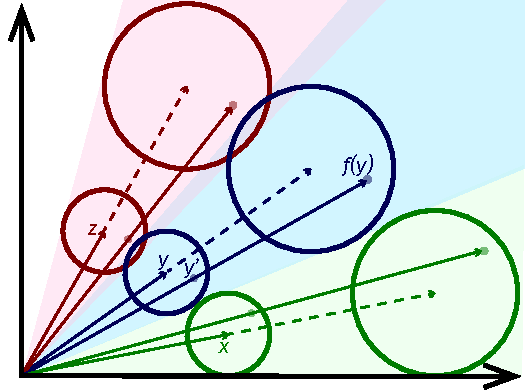
\includegraphics[width=0.5\columnwidth]{dcpe}
			\caption{Distance Comparison Preserving Encryption scheme \cite{dcpe}}%
		\end{figure}

	\end{frame}

	\begin{frame}{Search accuracy and TREC dataset}

		\begin{itemize}
			\item<1->
				Setup and query protocols: for given $\beta$
				\begin{itemize}
					\item Generate encryption key
					\item Encrypt dataset and queries set with $\beta$
					\item Run queries using conventional nearest-neighbor search (e.g., FAISS \cite{faiss})
					\item Report search accuracy metrics
				\end{itemize}

			\item<2->
				TREC 2020 dataset is 8.8M documents embedded with fine-tuned BERT \cite{bert} (768 dimensions) \\
				\begin{small}
					Thanks Hamed Zamani for the dataset
				\end{small}

			\item<3->
				Query is a 768-dimensional embedding asking for $k = \num{1000}$ closest documents \\
				\begin{small}
					TREC has set of documents, set of topics (questions), and relevance judgments (right answers)
				\end{small}

			\item<4->
				We report result set distance and difference, and ranking quality Recall, MRR and nDCG \\
				\begin{small}
					Set distance and difference measure pure \knn{} accuracy \\
					Recall, MRR and nDCG report ranking quality using relevance, common in informal retrieval literature
				\end{small}

		\end{itemize}

	\end{frame}

	\begin{frame}{Search accuracy results}

		\begin{figure}[h]
			\centering
			\includegraphics[width=0.7\textwidth]{knn-search}
			\caption{Rank quality metrics, result set distance and difference for $\beta \in \{ 0, 1, \ldots , 50 \} $}
		\end{figure}

	\end{frame}

	\section{Work-in-progress: \\ oblivious \texttt{JOIN}s}

	\begin{frame}{General idea}

		\begin{itemize}
			\item<1->
				Model: \alert{persistent}, query type: \alert{inner \texttt{JOIN}}

			\item<2->
				Input: two tables $T_1$ and $T_2$, query: return a cross product of $T_1$ and $T_2$ where $T_1.k = T_2.k$ \\
				\begin{small}
					We may also consider \texttt{SELECT JOIN}: \texttt{WHERE $T_1$.k = $T_2$.k AND $T_1$.a = 10}
				\end{small}

			\item<3->
				\alert{Challenge}: produce \texttt{JOIN} result hiding both access pattern and result size

			\item<4->
				\alert{Proposed solution}:
				\begin{itemize}
					\item use enclave (SGX) and oblivious primitives (sort, compaction)
					\item construct index over join keys, add DP noise to it
					\item partition the data by keys to fit a partition in the enclave
					\item consolidate sparse keys as an optimization
					\item do inner join within partition
				\end{itemize}

		\end{itemize}

	\end{frame}

	\begin{frame}{Detailed algorithm}

		\begin{itemize}
			\item<1->
				Construct list $L$ of the form $(k, n_1, \hat{n_1}, n_2, \hat{n_2})$, with an element per distinct key plus noise \\
				\begin{small}
					$k$ is a join key, $n$ and $\hat{n}$ are real and $\widehat{\text{noisy}}$ numbers of records with that key in corresponding input table \\
					Noise sampled to a hierarchical sanitizer from a Laplacian distribution
				\end{small}

			\item<2->
				Client \user{} sends sorted $L$ and hierarchical sanitizer over noise counts to the server \server{} \\
				\begin{small}
					Similar to \epsolute{}, adversary does not learn much from noisy counts
				\end{small}

			\item<3->
				Server $\server{}$ partitions $L$ by $k$, so that partition size ($\hat{n_1} + \hat{n_2}$) is bounded and uniform \\
				\begin{small}
					Resulting mapping from keys to partitions $\mathcal{M}(k) = i$ can be proven DP
				\end{small}

			\item<4->
				Consolidate sparse keys: ensure that each \emph{bin} corresponds to at least $U$ real keys \\
				\begin{small}
					\emph{Bin} is collection of tuples for which we will do cross product join
				\end{small}

			\item<5->
				Obliviously move and pad each bin/partition with dummy records \\
				\begin{small}
					Within each bin the data is sorted by input tables
				\end{small}

			\item<6->
				For each bin, \textbf{do cartesian product}

		\end{itemize}

	\end{frame}


	\maketitle

	\backupbegin%

	\ifthenelse%
		{\equal{\generatenotes}{only}}
		{\nocite{*}}
		{}

	\begin{frame}[allowframebreaks]{References}

		\bibliography{bibfile}

		\note{The references}

	\end{frame}

	\appendix

	\section{Appendix}

	\begin{frame}[label={frame:appendix:ore}]

		\frametitle{OPE / ORE schemes}

		\begin{adjustbox}{width=\linewidth}
			\begin{tabular}{ l c c c c c }

				\toprule

				\multirow{2}{*}{Scheme}						& \multicolumn{2}{c}{\onslide<1->{Primitive usage}}																						& \onslide<1->{Ciphertext size,}																& \onslide<1->{Leakage}																\onslide<1->{\\ \cline{2-3}}
				\rule{0pt}{10pt}							& \onslide<1->{Encryption}													& \onslide<1->{Comparison}									& \onslide<1->{or state size}																	& \onslide<1->{(in addition to inherent total order)}								\\

				\toprule

				BCLO~\cite{crypt-db-ope}					& \onslide<1->{$\bm{n}$ \textbf{HG}}										& \onslide<1->{none}										& \onslide<1->{$2n$}																			& \onslide<1->{\textbf{$\approx$ Top half of the bits}}								\\

				\midrule

				CLWW~\cite{practical-ore}					& \onslide<1->{$n$ PRF} 													& \onslide<1->{none}										& \onslide<1->{$2n$}																			& \onslide<1->{\textbf{Most-significant differing bit}}								\\

				\midrule

				\multirow{3}{*}{Lewi-Wu~\cite{lewi-ore}}	& \onslide<1->{\boldmath{} $\nicefrac{2n}{d}$ \unboldmath{} \textbf{PRP}}	& \onslide<1->{\multirow{3}{*}{$\frac{n}{2d}$ Hash}}		& \onslide<1->{\multirow{3}{*}{$\frac{n}{d} \left(\lambda + n + 2^{d + 1} \right) + \lambda$}}	& \onslide<1->{\multirow{3}{*}{Most-significant differing block}}					\\
															& \onslide<1->{$2 \frac{n}{d} \left( 2^d + 1 \right)$ PRF}					&															&																								&																					\\
															& \onslide<1->{$\frac{n}{d} 2^d$ Hash}										&															&																								&																					\\

				\midrule

				\multirow{3}{*}{CLOZ~\cite{adam-ore-v2}}	& \onslide<1->{$n$ PRF}														& \onslide<1->{\multirow{3}{*}{$\bm{n^2}$ \textbf{PPH}}}	& \onslide<1->{\multirow{3}{*}{$n \cdot h$}}													& \onslide<1->{\multirow{3}{*}{Equality pattern of most-significant differing bit}}	\\
															& \onslide<1->{$n$ PPH}														&															&																								&																					\\
															& \onslide<1->{1 PRP}														&															&																								&																					\\

				\midrule

				FH-OPE~\cite{fh-ope}						& \onslide<1->{1 Traversal}													& \onslide<1->{3 Traversals}								& \onslide<1->{$\bm{3 \cdot n \cdot N}$}														& \onslide<1->{Insertion order}														\\

				\bottomrule

			\end{tabular}
		\end{adjustbox}

		\hyperlink{frame:ore}{\beamerreturnbutton{Back to ORE}}

	\end{frame}

	\begin{frame}[label={frame:appendix:protocols}]

		\frametitle{Range query protocols}

		\begin{adjustbox}{width=\linewidth}
			\begin{tabular}{ l c c c c c c }

				\toprule

				\multirow{2}{*}{Protocol}						& \multicolumn{2}{c}{\onslide<1->{{\IO} requests}}																																& \multirow{2}{*}{\onslide<1->{Leakage}}	& \multicolumn{2}{c}{\onslide<1->{Communication (result excluded)}}																&	\onslide<1->{\\ \cline{2-3} \cline{5-6}}
				\rule{0pt}{10pt}								& \onslide<1->{Construction}									& \onslide<1->{Query}																							&											& \onslide<1->{Construction}									& \onslide<1->{Query} 											&	\\

				\toprule

				{\BPlus} tree with ORE							& \onslide<1->{$\log_B \frac{N}{B}$}							& \onslide<1->{$\log_B \frac{N}{B} + \frac{r}{B}$}																& \onslide<1->{\textbf{Same as ORE}}		& \onslide<1->{$1$}												& \onslide<1->{$1$}												&	\\
				\midrule

				Kerschbaum~\cite{florian-protocol}				& \onslide<1->{$\bm{\frac{N}{B}}$}								& \onslide<1->{$\log_2 \frac{N}{B} + \frac{r}{B}$}																& \onslide<1->{\textbf{Total order}}		& \onslide<1->{$\log_2 N$}										& \onslide<1->{$\log_2 N$}										&	\\

				\midrule

				POPE~\cite{pope} warm							& \multirow{2}{*}{\onslide<1->{$1$}}							& \onslide<1->{$\log_L \frac{N}{B} + \frac{r}{B}$}																& \onslide<1->{\textbf{Partial order}}		& \multirow{2}{*}{\onslide<1->{$1$}}							& \onslide<1->{$\log_L N$}										&	\\

				POPE~\cite{pope} cold							& 																& \onslide<1->{$\bm{{\nicefrac{N}{B}}}$}																		& \onslide<1->{Fully hiding}				& 																& \onslide<1->{$\bm{N}$}										&	\\

				\midrule

				Logarithmic-BRC~\cite{practical-range-search}	& \onslide<1->{\textbf{---}}									& \onslide<1->{$\bm{r}$}																						& \onslide<1->{Same as SSE}					& \onslide<1->{\textbf{---}}									& \onslide<1->{$\log_2 N$}										&	\\

				\midrule

				\multirow{2}{*}{ORAM}							& \multirow{2}{*}{\onslide<1->{$\bm{{ \log^2 \frac{N}{B} }}$}}	& \multirow{2}{*}{\onslide<1->{$\bm{{ \log_2 \frac{N}{B} \left( \log_B \frac{N}{B} + \frac{r}{B} \right) }}$}}	& \onslide<1->{Fully hiding}				& \multirow{2}{*}{\onslide<1->{$\bm{{ \log^2 \frac{N}{B} }}$}}	& \multirow{2}{*}{\onslide<1->{$\bm{{ \log^2 \frac{N}{B} }}$}}	&	\\
																&																&																												& \onslide<1->{(access pattern)}			&																&																&	\\

				\bottomrule

			\end{tabular}
		\end{adjustbox}

		\hyperlink{frame:ore}{\beamerreturnbutton{Back to ORE}}

	\end{frame}

	\begin{frame}[label={frame:appendix:plot}]

		\frametitle{One of the experimental results}

		\begin{figure}[h]
			\centering
			\includegraphics[width=0.6\textwidth]{protocol-charts-qios}
			\caption{
				Query stage number of I/O requests \\
				\hyperlink{frame:ore}{\beamerreturnbutton{Back to ORE}}
			}
		\end{figure}

	\end{frame}

	\begin{frame}[label={frame:appendix:oram}]

		\frametitle{Access pattern and ORAM}

		\justifying%

		\textbf{Access pattern} is a sequence of memory accesses \oramProgram{}, where each access consists of the memory \emph{location} $o$, read \oramRead{} or write \oramWrite{} \emph{operation} and the \emph{data} $d$ to be written.

		Oblivious RAM (ORAM) is a mechanism that hides the accesses pattern.
		More formally, \oram{} is a protocol between the client \client{} (who accesses) and the server \server{} (who stores), with a guarantee that the view of the server is indistinguishable for any two sequences of the same lengths.

		\begin{columns}[T]
			\column{0.475\textwidth}

				\[
					\begin{split}
						\abs{\oramProgram_1}					& = \abs{\oramProgram_2}							\\
						\textsc{View}_\server (\oramProgram_1)	& \cindist \textsc{View}_\server (\oramProgram_2)
					\end{split}
				\]

			\column{0.475\textwidth}

				\procedure[linenumbering]{\oram{} protocol}{
					\textbf{Client \client}											\>														\> \textbf{Server \server}	\\
					%
					\oramProgram{} = \left. (\oramRead, i, \bot) \right|_{i = 1}^5	\> 														\>							\\
					%
					\text{(client state)}											\> \sendmessageboth*[6em]{\algo{ORAM}{\oramProgram}}	\> \text{(server state)}	\\
					%
					\{ d_1, d_2, d_3, d_4, d_5 \}									\>														\>
				}

		\end{columns}

		\vspace*{1ex}

		For example: Square Root ORAM~\cite{oram-theory}, Hierarchical ORAM~\cite{oram-original}, Binary-Tree ORAM~\cite{binary-tree-oram}, Interleave Buffer Shuffle Square Root ORAM~\cite{shortest-path-oram}, TP-ORAM~\cite{tp-oram}, \textbf{Path-ORAM}~\cite{path-oram} and TaORAM~\cite{taostore}.
		\alert{ORAM incurs at least logarithmic overhead in the number of stored records.~\cite{oram-original}}
		\hyperlink{frame:epsolute-motivation}{\beamerreturnbutton{Back to \epsolute{}}}

	\end{frame}

	\begin{frame}[label={frame:appendix:dcpe}]

		\frametitle{Component: DCPE}

		\[
			\forall x, y, x \in \mathbb{X} : \algo{Dist}{x, y} < \algo{Dist}{x, z} - \beta \implies \algo{Dist}{f(x), f(y)} < \algo{Dist}{f(x), f(z)}
		\]

		\begin{itemize}
			\item<1->
				The scheme is by Riddhi Ghosal and Adam O'Neil
			\item<2->
				\textbf{Key generation}: sample at random length multiplier $s$ and seeds for samplers $K$
			\item<3->
				\textbf{Encrypt}: take input vector $x \in \RR^d$
				\begin{itemize}
					\item Sample nonce $n$
					\item Using nonce and seeds, sample a point $a$ on a $\beta$-radius $d$-dimensional ball
					\item New vector is extended times $s$ and points to $a$
				\end{itemize}
			\item<4->
				\textbf{Decrypt}: take encrypted vector $c \in \RR^d$ and nonce $n$
				\begin{itemize}
					\item Do same steps except \emph{shrink} times $s$ and \emph{remove} ball component
				\end{itemize}
		\end{itemize}

		\hyperlink{frame:knn}{\beamerreturnbutton{Back to \knn{}}}

	\end{frame}

	\begin{frame}[label={frame:appendix:trec-faiss}]

		\frametitle{Component: TREC dataset and FAISS~\cite{faiss}}

		\begin{itemize}
			\item<1->
				Dataset is 8.8M documents represented as vectors of 768 dimensions \\
				\begin{small}
					Thanks Hamed Zamani for the dataset
				\end{small}

			\item<2->
				Query is a 768-dimensional vector asking for $k = 1000$ closest (inner product) documents

			\item<3->
				% cspell:disable-next-lin
				Original document set is a \textbf{T}ext \textbf{RE}trieval \textbf{C}onference (TREC) test collection \\
				\begin{small}
					set of documents, set of topics (questions), and corresponding set of relevance judgments (right answers)
				\end{small}

			\item<4->
				FAISS~\cite{faiss}: GPU-enabled library for efficient similarity search and clustering of dense vectors
				\begin{small}
					Developed and maintained by Facebook AI
				\end{small}

			\item<5->
				General algorithm: for different $\beta$
				\begin{itemize}
					\item Encrypt dataset with $\beta$
					\item Encrypt queryset with $\beta$
					\item Run queries with FAISS
					\item Generate TREC metrics (using relevance judgments)
				\end{itemize}

		\end{itemize}

		\hyperlink{frame:knn}{\beamerreturnbutton{Back to \knn{}}}

	\end{frame}

	\begin{frame}[label={frame:appendix:knn-plot}]

		\frametitle{Intermediate results}

		\begin{figure}[h]
			\centering
			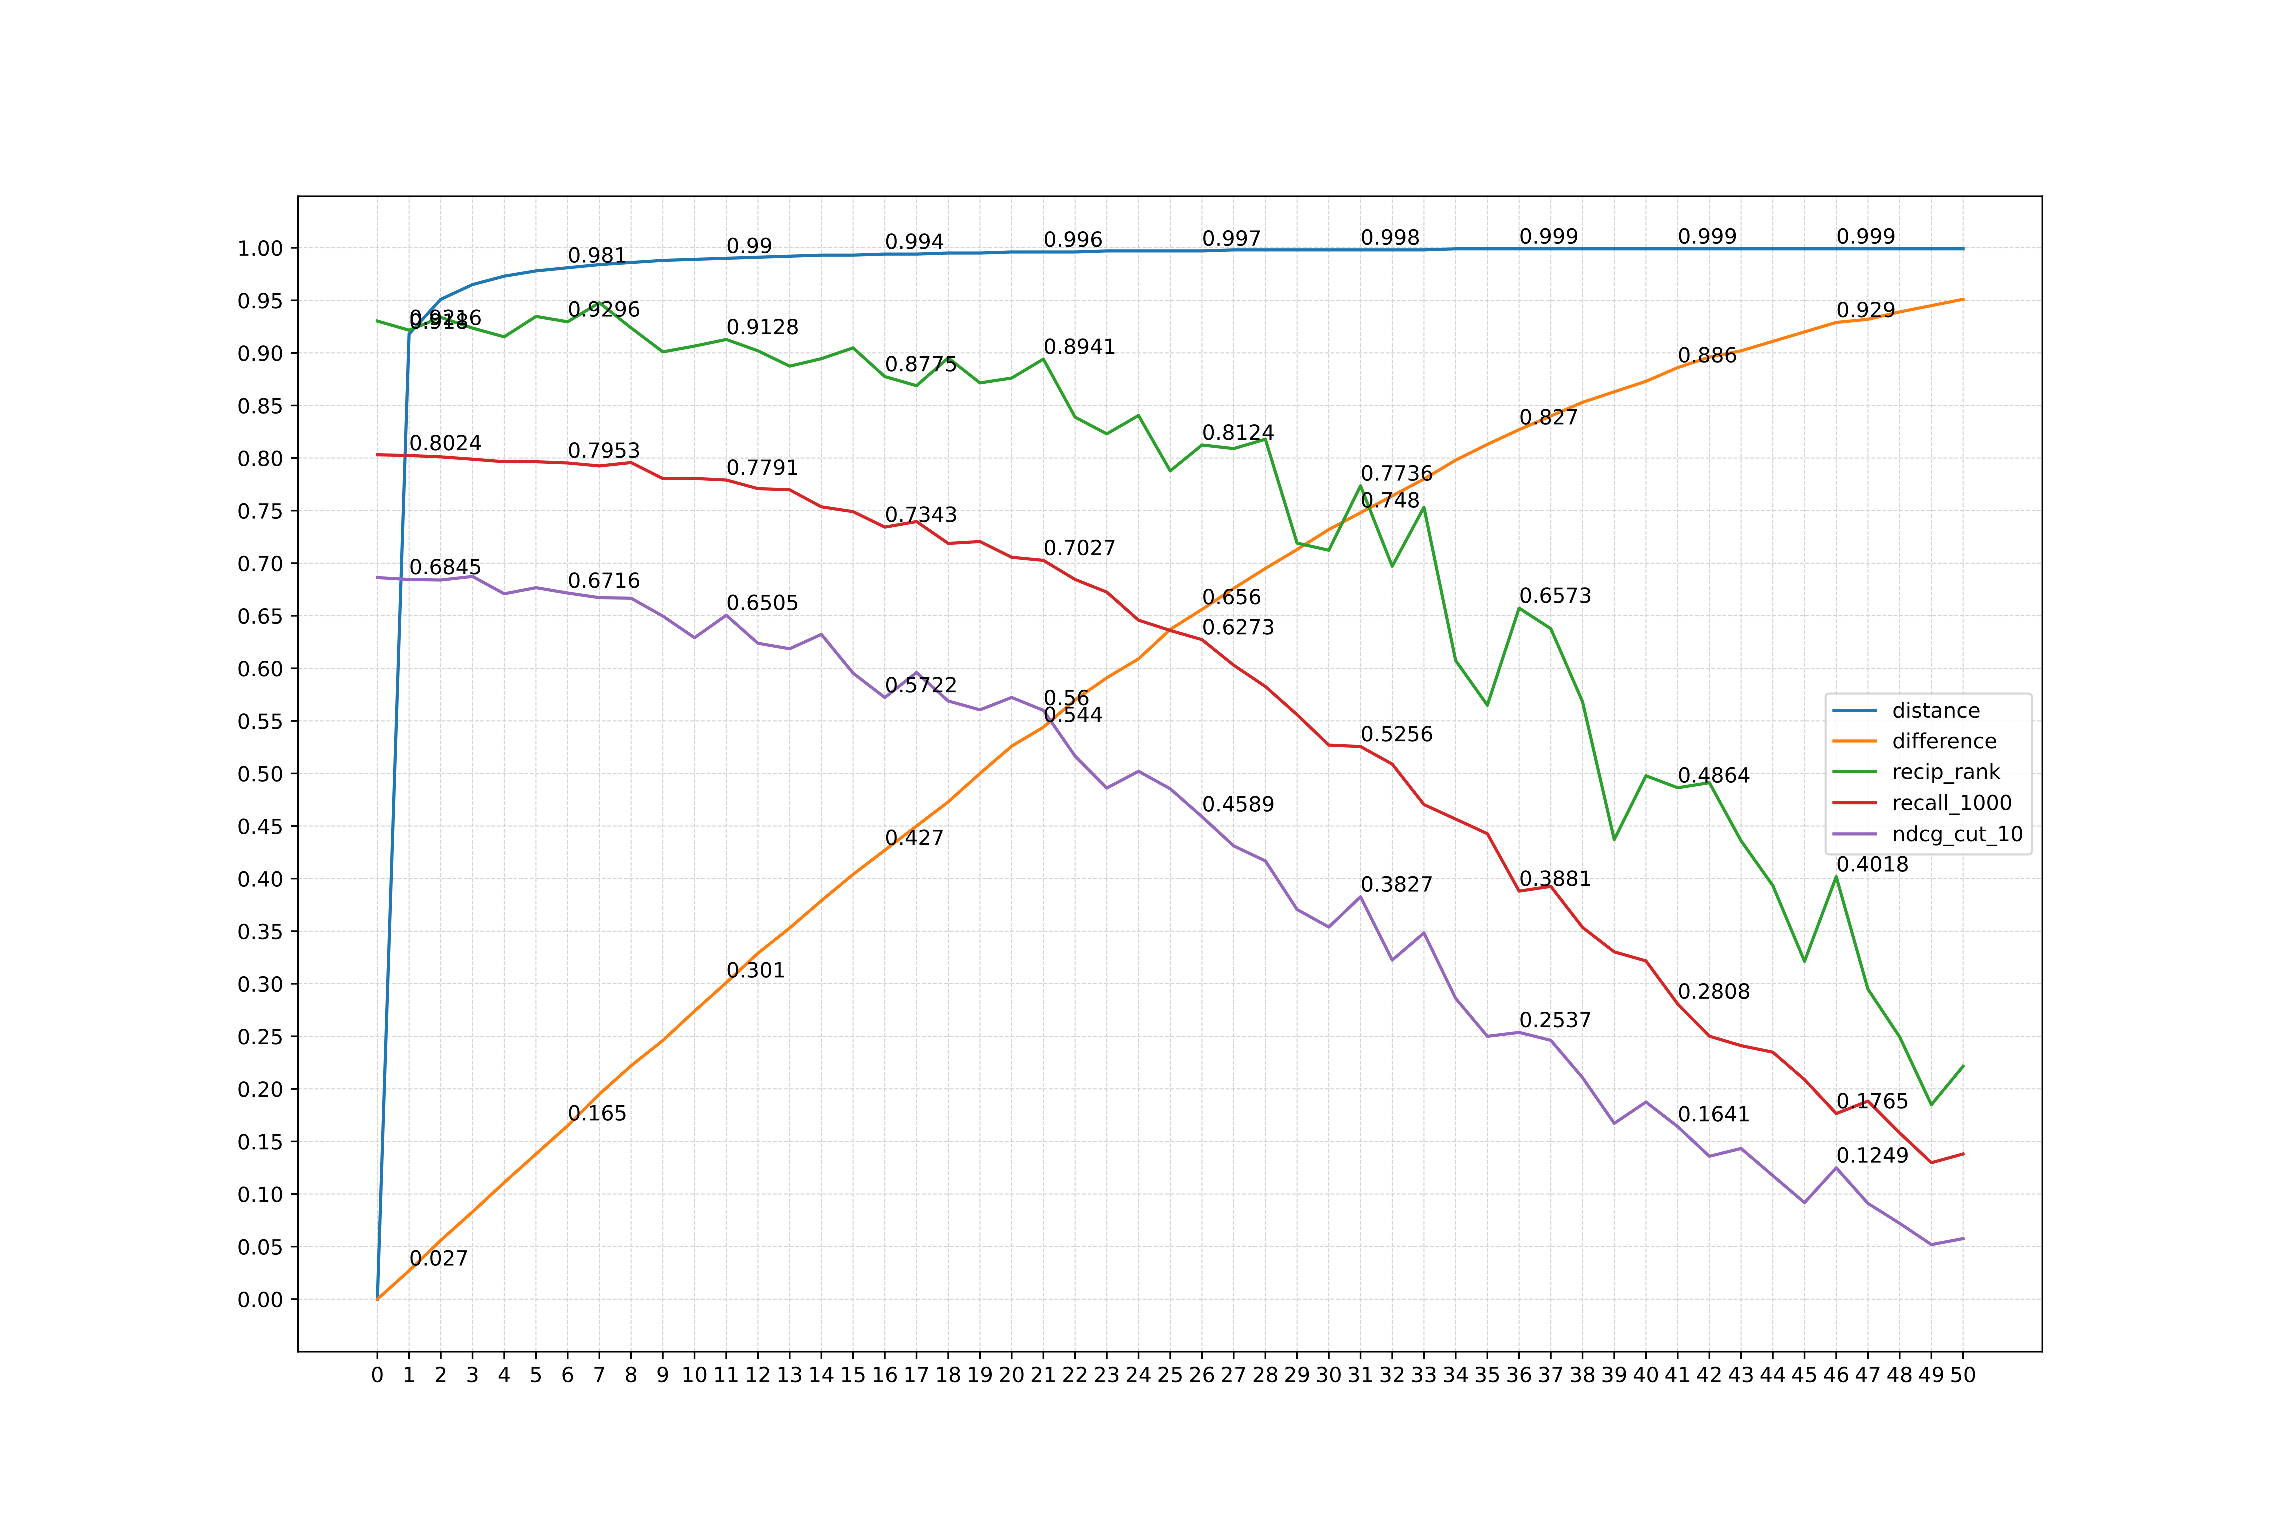
\includegraphics[trim=60 60 60 60,clip,width=0.75\textwidth]{knn}
			\caption{
				TREC metrics, result set distance and difference, for running \knn{} search for $\beta \in \{ 0, 1, \ldots , 50 \} $ \\
				\hyperlink{frame:knn}{\beamerreturnbutton{Back to \knn{}}}
			}
		\end{figure}

	\end{frame}

	\begin{frame}[label={frame:appendix:joins-detailed}]

		\frametitle{Oblivious \texttt{JOIN}s detailed algorithm}

		\begin{itemize}
			\item<1->
				Construct list $L$ of the form $(k, n_1, \hat{n_1}, n_2, \hat{n_2})$, with an element per distinct key plus noise \\
				\begin{small}
					$k$ is a join key, $n$ and $\hat{n}$ are real and $\widehat{\text{noisy}}$ numbers of records with that key in corresponding input table \\
					Noise sampled to a hierarchical sanitizer from a Laplacian distribution
				\end{small}

			\item<2->
				Client \user{} sends sorted $L$ and hierarchical sanitizer over noise counts to the server \server{} \\
				\begin{small}
					Similar to \epsolute{}, adversary does not learn much from noisy counts
				\end{small}

			\item<3->
				Server $\server{}$ partitions $L$ by $k$, so that partition size ($\hat{n_1} + \hat{n_2}$) is bounded and uniform \\
				\begin{small}
					Resulting mapping from keys to partitions $\mathcal{M}(k) = i$ can be proven DP
				\end{small}

			\item<4->
				Consolidate sparse keys: ensure that each \emph{bin} corresponds to at least $U$ real keys \\
				\begin{small}
					\emph{Bin} is collection of tuples for which we will do cross product join
				\end{small}

			\item<5->
				Obliviously move and pad each bin/partition with dummy records \\
				\begin{small}
					Within each bin the data is sorted by input tables
				\end{small}

			\item<6->
				For each bin, \textbf{do cartesian product}

		\end{itemize}

		\hyperlink{frame:oblivious-joins}{\beamerreturnbutton{Back to Oblivious Joins}}

	\end{frame}


	\backupend%

\end{document}
